\documentclass[pdftex,12pt,letter]{article}
\usepackage{fancyhdr}
\usepackage{enumerate}
\usepackage{tabularx}
\usepackage{graphicx}
\usepackage{array}
\usepackage[justification=justified,singlelinecheck=false]{caption}
\usepackage{placeins}
\pagestyle{fancy}
\makeatletter
  \renewcommand\@seccntformat[1]{\csname the#1\endcsname.\quad}
\makeatother

\newcolumntype {Y}{ >{\raggedright \arraybackslash }X}
\newcommand{\HRule}{\rule{\linewidth}{0.5mm}}
\captionsetup{labelformat=empty}

\begin{document}

\begin{titlepage}
\begin{flushright}
\HRule \\[0.4cm]
{ \bfseries
{\huge Design Document\\[1cm]}
{\Large for\\[1cm]}
{\huge CWRUtility\large\\[4cm]}
{\large Prepared by\\Jason Kuster, Stuart Long, and William Ordiway\\[1cm]
Version 1.0 initial\\[1cm]
KOALAA Development\\[1cm]
October 6, 2012}}
\end{flushright}
\end{titlepage}
\tableofcontents{}
\begin{table}[!t]
\caption*{\bfseries Revision History}
\begin{tabularx}{\textwidth }[t]{|l|Y|Y|l|}
\hline
\bfseries Name & \bfseries Date & \bfseries Reasons for Change & \bfseries Version \\ \hline
Long & 10/6/2012 & Initial Outline & 1.0 initial\\
\hline
\end{tabularx}
\end{table}
\FloatBarrier
\newpage
\clearpage
\section{Overview}
\subsection{Overall Design}
The \emph{CWRUtility} application is essentially a collection of CWRU-related features that allows for easy, centralized access to each of the features. The complete list of features and their description can be found in the \emph{CWRUtility} SRS. Since this software system can be easily broken down into separate, uncoupled features, the design of the overall system is also broken down. Each feature will have it's own design, documented below in the "Features" section, that will operate independently of the other features. The only exception to this rule is the "StartPage" feature, which can also be seen as the overall application manager. Explained in detail below, the "StartPage" feature will be responsible for navigating the system to the different features and controlling any communication between the features. The figure below shows the various components of the system and how they are linked. This diagram could be seen as the highest level of design for the system.
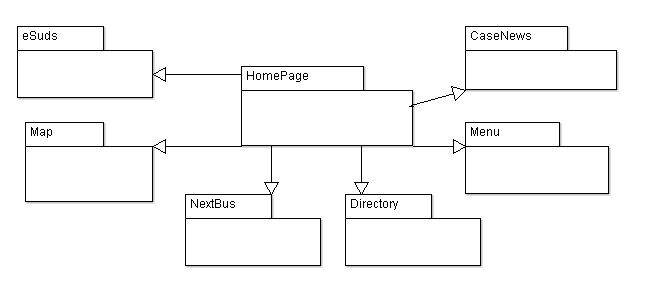
\includegraphics[width=120mm]{OverallCD.png}
\subsection{User Interface}
The implementation of any user interfaces on the Windows Phone 7/8 platform is done using the eXtensible Application Markup Language (XAML). Essentially, XAML can be used as a layout language similar to HTML. XAML provides a straightforward way to generate, lay out, and populate the on-screen elements. Data population will be done by using Model View View-Model (MVVM), a data-binding interface built into the Windows Phone SDK. The data fields will be laid out in XAML, which will comprise the view; the code to map the data to the view is contained in the view-model, and the raw data will be stored in application storage.It is important to note that a markup language is very dissimilar to a programming language as it works through simply creating a series of attributes and assigning values to them. The Windows Phone OS actually handles creating the UI based on these attributes, therefore this software system does not have to.
\\
\section{Features}
\subsubsection{StartPage}
The "StartPage" feature represents both the manager for the rest of the application and the feature the user is taken to on application start-up. This feature actually comprises two different application pages for the "At-a-glance" page and one for the page listing the full list of features.
\subsection{Class Diagram}
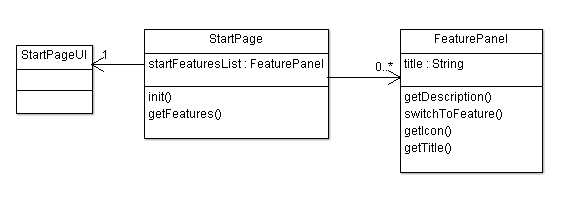
\includegraphics[width=120mm]{StartPageCD.png}
\subsubsection{StartPage}
The StartPage class will be the main class in this feature. It will be the feature that opens when the user starts the application, an operation that is handled by the XAML (UI) file. The page will display the application title at the top, then the feature title below that, and finally a scrollable list of featurePanels. Each featurePanel will represent one of the other features within the application and will display the feature title as well as a potentially "live" description for that feature. For example, one of the features in this feature panel will be the "nextBus" feature, and its feature panel will display the next shuttle time for the user's last selected stop. This page is intended to display the most commonly used feature for a user-friendly way to get to those applications. The features that will be displayed on this page are the "nextBus", "caseNews", "eSuds", and.....If the user clicks on a feature panel, the application will switch the user to that feature.


\subsection{Map}
The "Map" feature will allow the users to view a map of the Case Western Reserve University Campus. The feature will use the interactive map controller provided by the Windows Phone SDK. This map controller is the same map controller used for the default Windows Phone 7 map application. Since the map controller is already provided by the Windows Phone SDK, this feature will have a simple design.
\subsubsection{Class Diagram}
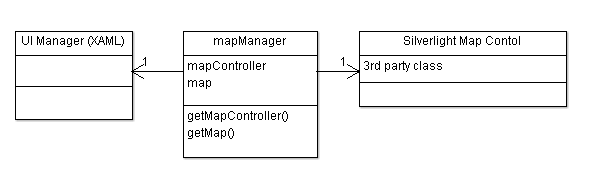
\includegraphics[width=120mm]{MapCD.png}
\subsubsection{SilverlightMapControl}
The SilverlightMapControl class is part of a third party library provided by Microsoft Corporation. It provides basic map controls such as zooming in, zooming out, and panning for any provided map. The MapManager will simply send a saved map of the CWRU campus to the map controller.
\subsubsection{MapManager}
The MapManager class is responsible for handling the other two classes: the SilverlightMapControl and the UI manager. It will have a saved copy of the CWRU map that it will send to the SilverlightMapControl. It will also be responsible for sending the SilverlightMapControl to the UI manager so that the UI manager can display the map.
\subsubsection{UIManager}
The UIManager for this feature will not be a true class, since all UI for Windows Phone is done using XAML files. Still, this manager will be responsible for laying out the components of the feature. Namely, it will have to layout the title of the application at the top, the name of this feature below that, and the actual map will take up most of the application. The XAML file will be sent the map controller (along with that map controller's view, i.e. the map)  by the MapManager.
%william's section
\subsection{Directory}
The "Directory" feature will allow users to view the location, hours, phone number, and a description of the wide assortment of Case Western Reserve University campus resources. This feature will be simple in design because besides presenting preloaded information its only function is to facilitate calling campus resources 
\subsubsection{Class Diagram}
\begin{flushleft}
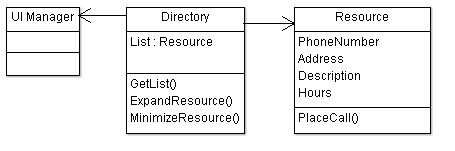
\includegraphics[width=120mm]{DirectoryCD.png}
\end{flushleft}
\subsubsection{Class Descriptions: Resource}
Each campus resource that will be represented in our application will be represented as an object in the resource class possessing a Phone Number, an Address, open hours, and a brief description about what the resource can be used for. The address, open hours, and description will all be simbple text variables which are displayed on screen. However the phone number variable is tied to the PlaceCall() operation. By tapping the phone number of a resource the users phone will place a call to that number.
\subsubsection{Class Description: Directory}
The directory class is used to maintain a variable List which contains a number of resource objects, each of which represent a different campus resource.
\subsubsection{Class Description: UI Manager}
The UIManager for this feature will not be a true class, since all UI for Windows Phone is done using XAML files. Still, this manager will be responsible for laying out the components of the feature. Namely, it will have to layout the title of the application at the top, the name of this feature below that. Taking up the majority of the screen though will be a scrollable alphabetized list of campus resources. Selecting a campus resource will expand information about that resource and shut the previous, if any, selected resource.


\subsection{NextBus}
The "NextBus" feature will allow the users to interface with the NextBus, Inc. bus times prediction website. This feature will offer users the ability to select bus routes, bus direction, and stops in order to facilitate the use of the "Greenie" bus system on campus. The feature's main page will be a single Windows Phone-style page with three drop-down selection boxes and a "Go" button. There will be a field, initially blank, which will populate with the next prediction times (max 3). Additionally, the NextBus section will feature on the main page, where it will provide a small icon which contains the stop which the user has marked as a "favorite".
\subsection{Class Diagram}
\subsection{Class Descriptions}
\subsubsection{BusScheduleManager}
%\subsection{Schedule}
%The "Schedule" feature will allow users to add classes or custom events to a saved schedule on the system. This feature will require three classes: a schedule event, a schedule event manager to handle schedule events, and a UI manager for the schedule.
\lfoot{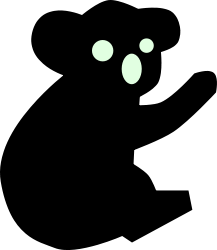
\includegraphics[height=1cm]{DarkKoala.png}}

%\subsection{Class Diagram}
%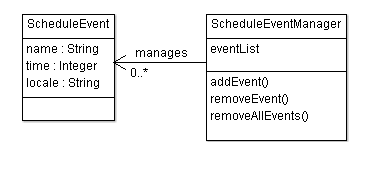
\includegraphics[width=80mm]{ScheduleEventsCD.png}
%\figurename{Schedule Class Diagram}
%\subsection{Class Descriptions}
%The following class descriptions describe the above class diagram.
%\subsubsection{ScheduleEvent}
\end{document}
